% -*- coding: UTF-8 -*-
% vim: autoindent expandtab tabstop=4 sw=4 sts=4 filetype=tex
% vim: spelllang=de spell
% chktex-file 27 - disable warning about missing include files

\subsection{Operationen für implizite Oberflächen}
\label{subsec:implicit_surfaces_ops}

Um mit impliziten Oberflächen nicht nur einfache Objekte wie
beispielsweise eine Kugel darstellen zu können muss man diese auch
transformieren können.

Wie~\citeauthor{hart_sphere_1994} beschreibt, werden implizite
Oberflächen durch die Invertierung des Raumes, in welchem sich eine
Oberfläche befindet, transformiert~\parencite[S. 543]{hart_sphere_1994}.
Der Raum, in dem sich eine implizite Oberfläche befindet, ist die Domäne
der impliziten Funktion der Oberfläche.

Sei $T(\bm{x})$ eine Transformation und $f(\bm{x})$ eine Distanzfunktion,
welche eine implizite Oberfläche definiert. Somit ist die transformierte
implizite Oberfläche~\parencite[S. 534]{hart_sphere_1994}:

\begin{gather}
    f(T^{-1}(\bm{x})) = 0
\end{gather}

Bei Transformationen handelt es sich um von dem Vorzeichen abhängige
Distanzfunktionen (\textit{signed distance functions}).

Es werden folgende Arten von Transformationen
unterschieden~\parencite[S. 14]{hart_ray_1993}:
\begin{itemize}
    \item{Distanz-Operationen}\\
        Zum Beispiel Vereinigung, Subtraktion oder Intersektion.
    \item{Domänen-Operationen}\\
        Zum Beispiel Wiederholung, Rotation, Translation und Skalierung.
    \item{Distanz-Deformationen}\\
        Zum Beispiel Versatz (displacement) und Vermengung/Vermischung.
        (\textit{blend})
    \item{Domänen-Deformationen}\\
        Zum Beispiel ``Verwindung'' (\textit{twist}) und Biegung
        (\textit{bend}).
\end{itemize}

\subsubsection{Isometrien}
\label{ssubsec:implicit_surfaces_ops_isometries}

Nicht alle Transformationen erhalten dabei die Distanz, welche die
Distanzfunktion der transformieren Oberfläche zurückgeben würde. In
solch einem Falle ist die zurückgegebene Distanz nicht die Distanz eines
beliebigen Punktes im Raum zu dem ihm nächsten Punkt einer impliziten
Oberfläche.

Transformationen, welche die Distanz hingegen erhalten,
bezeichnet~\citeauthor{hart_sphere_1994}
als~\textit{Isometrien}~\parencite[S. 534]{hart_sphere_1994}. Dazu
zählen Rotationen, Translationen aber auch Reflexionen.

Ist $\bm{I}$ eine Isometrie, dann benötigt die zurückgegebene Distanz der
Distanzfunktion $f(\bm{x})$ \textit{keine Anpassung}.

\begin{gather}
    d(\bm{x}, \bm{I} \circ f^{-1}(0)) = d(\bm{I}^{-1}(\bm{x}), f^{-1}(0))
\end{gather}

Dabei ist $\bm{I}$ eine Isometrie und $f^{-1}(0)$ eine implizite
Oberfläche.

\subsubsection{Uniforme Skalierung}
\label{ssubsec:implicit_surfaces_ops_scaling}

Eine Skalierung bewahrt keine Distanzen. Somit muss die zurückgegebene
Distanz einer Distanzfunktion entsprechend angepasst werden.

\citeauthor{hart_sphere_1994} gibt die uniforme Skalierung als
Transformation $\bm{S(x)}$  der folgenden Form an~\parencite[S. 534]{hart_sphere_1994}:

\begin{gather}
    \bm{S(x)} = s \cdot \bm{x}
\end{gather}

Dabei ist $s$ der Skalierungsfaktor. Die Invertierung der Skalierung
ist gegeben als~\parencite[S. 534]{hart_sphere_1994}:

\begin{gather}
    \bm{S^{-1}(x)} = {1 \over s} \cdot \bm{x}
\end{gather}

Somit ist die Distanz zu der skalierten impliziten
Oberfläche~\parencite[S. 534]{hart_sphere_1994}:

\begin{gather}
    d(\bm{x}, \bm{S}(f^{-1}(0))) = s \cdot d(\bm{S}^{-1}(\bm{x}), f^{-1}(0))
\end{gather}

Dabei wird die von der Distanzfunktion der skalierten impliziten Oberfläche
zurückgegebene Distanz mit dem Skalierungsfaktor $s$ multipliziert, was die
eigentliche Information der Distanz erhält und die Skalierung somit isometrisch
macht.

\subsubsection{``Verwindung'' (\textit{Twist})}
\label{ssubsec:implicit_surfaces_ops_twist}

Gemäss~\citeauthor{hart_sphere_1994} werden bei der ``Verwindung''
(\textit{Twist}) einer impliziten Oberfläche zwei Achsen (z.B. $x$ und
$y$) anhand einer linearen Funktion $a(\cdot)$ in Abhängigkeit der
dritten Achse (z.B. $z$) rotiert~\parencite[S. 543]{hart_sphere_1994}:

\begin{gather}
    twist(\bm{x}) = \begin{pmatrix} 
        x \cdot \cos{a(z)} - y \cdot \sin{a(z)},\\
        x \cdot \sin{a(z)} + y \cdot \cos{a(z)},\\
        z
    \end{pmatrix}
\end{gather}

\subsubsection{Vereinigung}
\label{ssubsec:implicit_surfaces_ops_union}

Die Vereinigung zweier impliziter Oberflächen $A$ und $B$ wird
von~\citeauthor{hart_sphere_1994} als minimale Distanz der jeweiligen,
vom Vorzeichen abhängigen Distanzfunktion $f_{A}$ respektive $f_{B}$
definiert~\parencite[S. 531 bis 532]{hart_sphere_1994}:

\begin{gather}
    d(\bm{x}, A \cup B) = \min(f_{A}(\bm{x}), f_{B}(\bm{x}))
\end{gather}

Dabei $\bm{x}$ den abzutastenden Punkt im Raum darstellt.

Wie~\citeauthor{hart_sphere_1994} schreibt, ist die Distanz zu einer
Menge von Objekten die kürzeste der Distanzen zu jedem der
zusammengesetzten Objekte~\parencite[S. 531 bis 532]{hart_sphere_1994}.

Somit erlaubt die Vereinigung die Kombination von mehreren impliziten
Oberflächen, ohne dass diese miteinander in Kontakt stehen. So kann
beispielsweise eine komplexe Szene modelliert werden.

\begin{figure}[H]
    \centering
    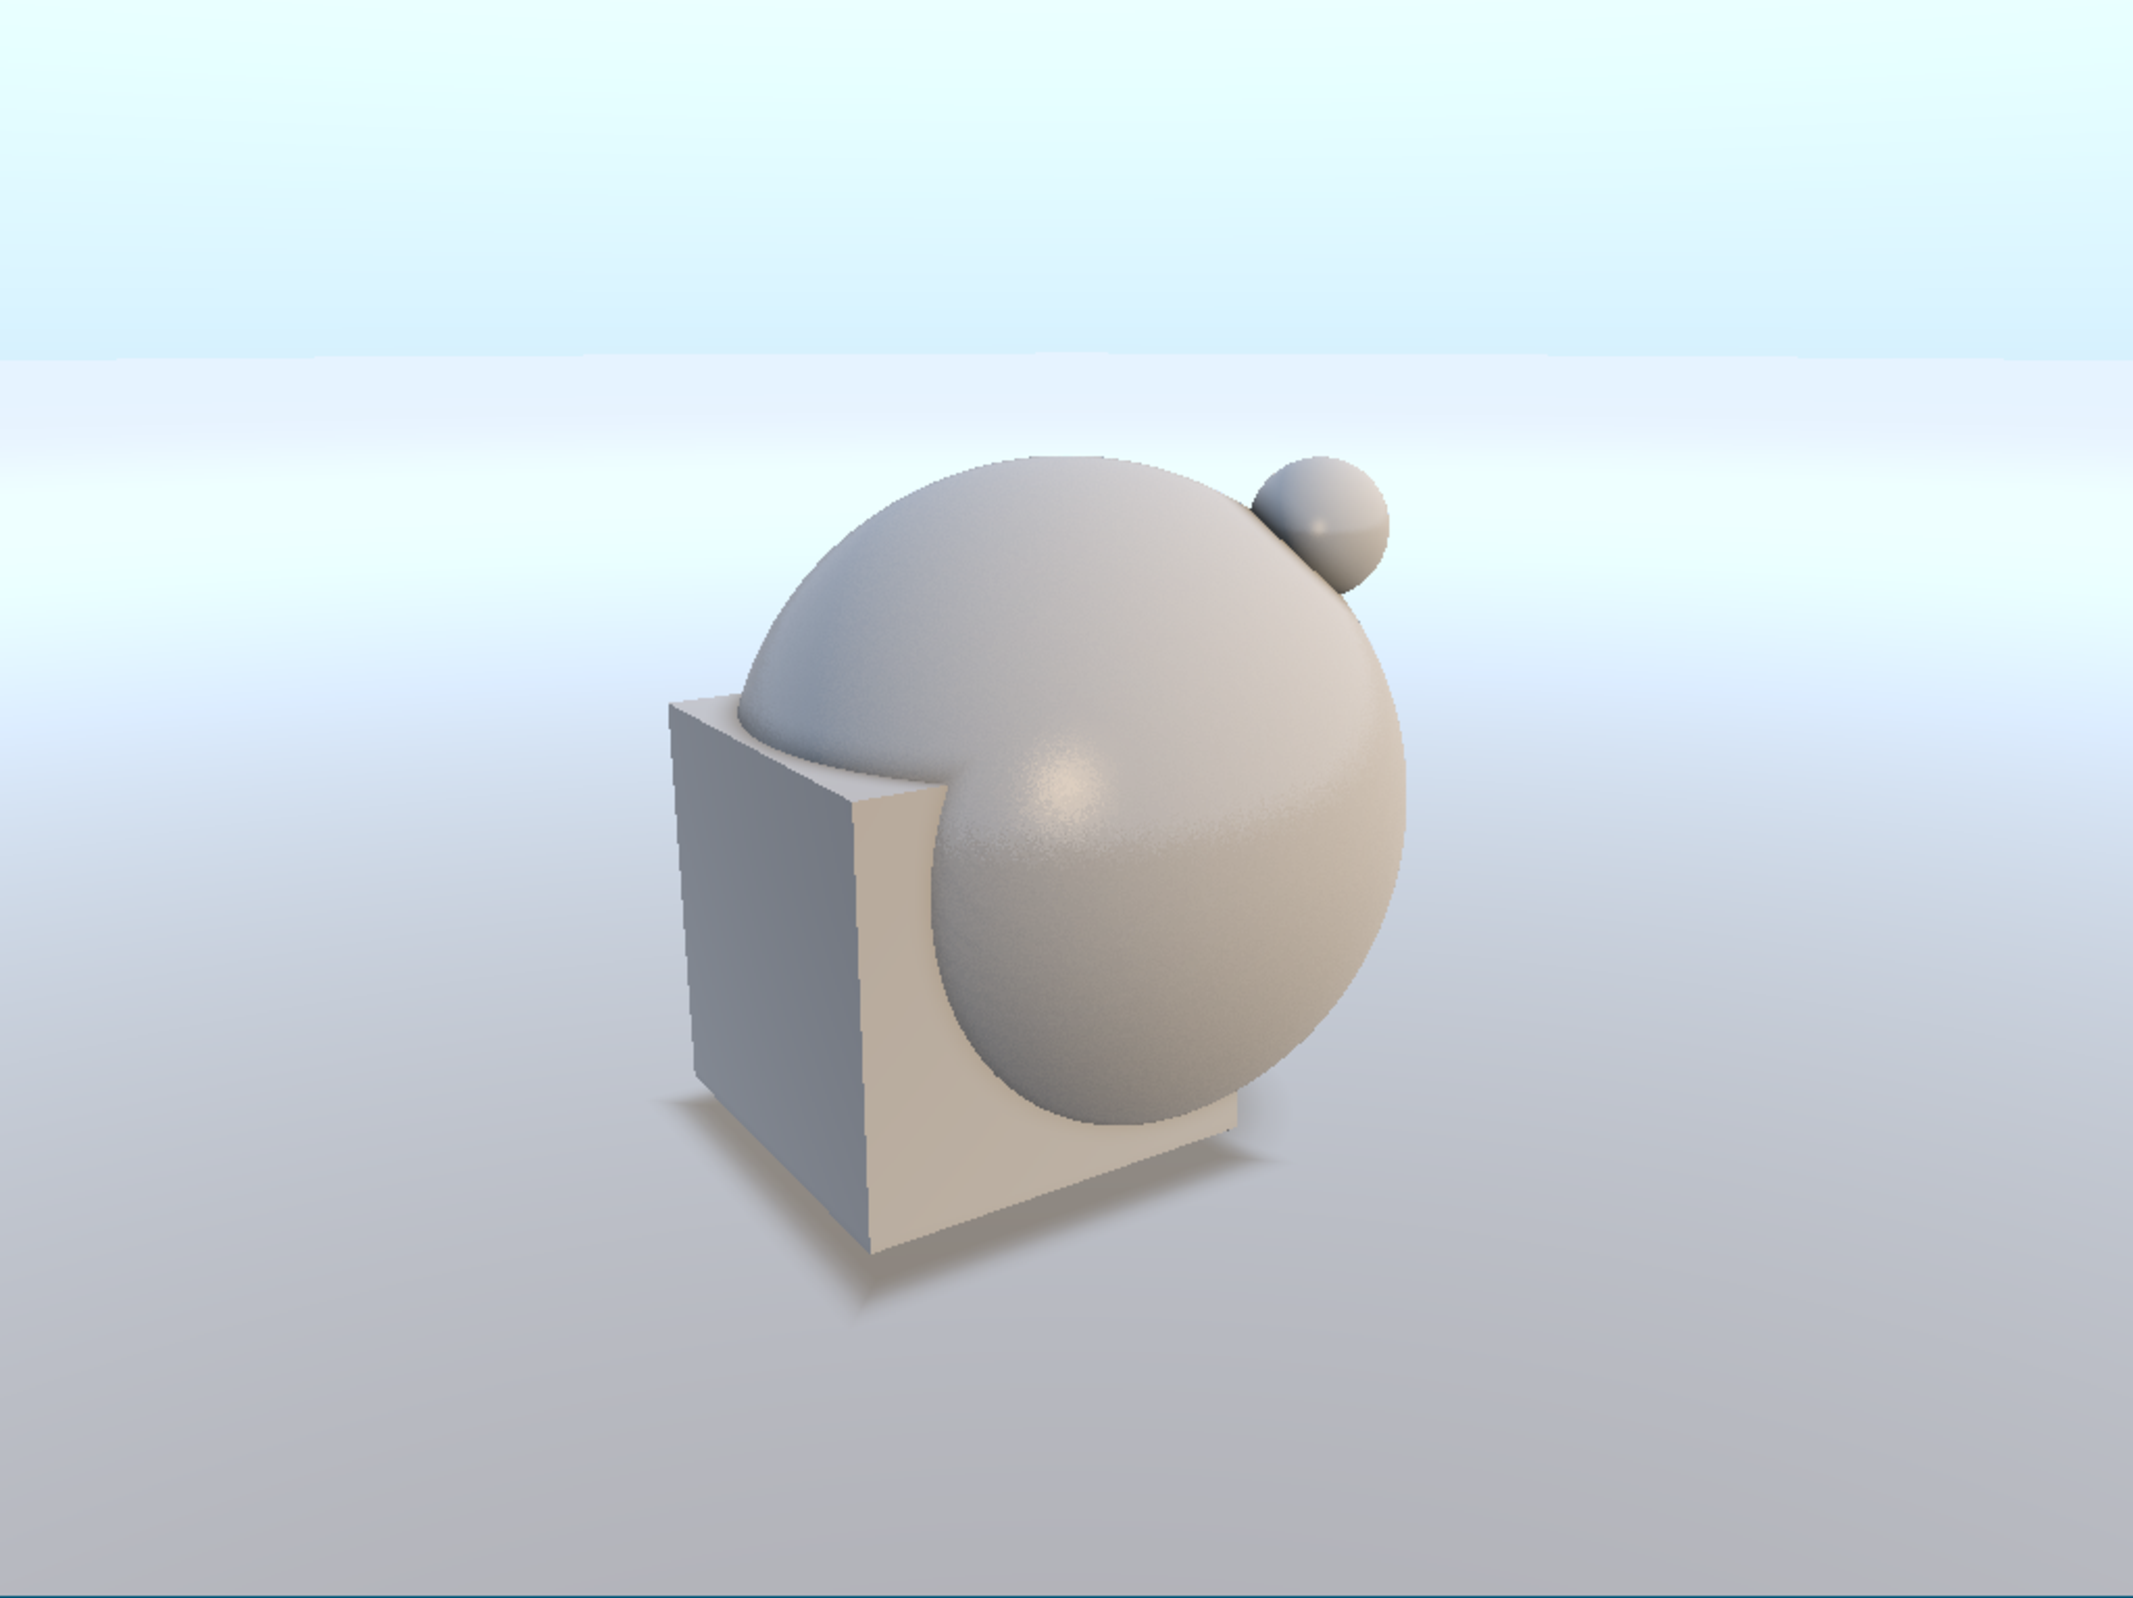
\includegraphics[width=0.5\textwidth]{img/sphere_tracing_union.pdf}
    \caption{Vereinigung von zwei Kugeln und einem Würfel. Bei dem
        Untergrund der Szene handelt es sich um eine Ebene, welche mit dem
        Rest der Szene vereinigt wird.\protect\footnotemark}\label{
        fig:implicit_surfaces_ops_union}
\end{figure}
\footnotetext{Eigene Darstellung}

\subsubsection{Subtraktion}
\label{ssubsec:implicit_surfaces_ops_subtraction}

Für die Subtraktion wird die Distanz zum Komplement eines Objektes
$\bm{A}$ verwendet. Dabei wird die Eigenschaft der Abhängigkeit vom 
Vorzeichen der entsprechenden Distanzfunktionen genutzt~\parencite[S.
532]{hart_sphere_1994}:

\begin{gather}
    d(\bm{x}, \mathbb{R}^{3} \setminus A) = -f_{A}(\bm{x})
\end{gather}

Somit kann die Subtraktion zweier impliziter Oberflächen $A$ und $B$
gemäss~\citeauthor{hart_sphere_1994} als Intersektion eines Objektes $A$ mit der
Subtraktion des Raumes bzw.\ der Domäne mit einem Objekt $B$ angesehen werden,
daher folgt~\parencite[S. 532]{hart_sphere_1994}:

\begin{align}
    d(\bm{x}, A - B) &= A \cap (\mathbb{R}^{3} \setminus B) \\
                     &\geq \max(f_{A}(\bm{x}), -f_{B}(\bm{x}))
\end{align}

Dabei stellt $\bm{x}$ den abzutastenden Punkt im Raum dar.

\begin{figure}[H]
    \centering
    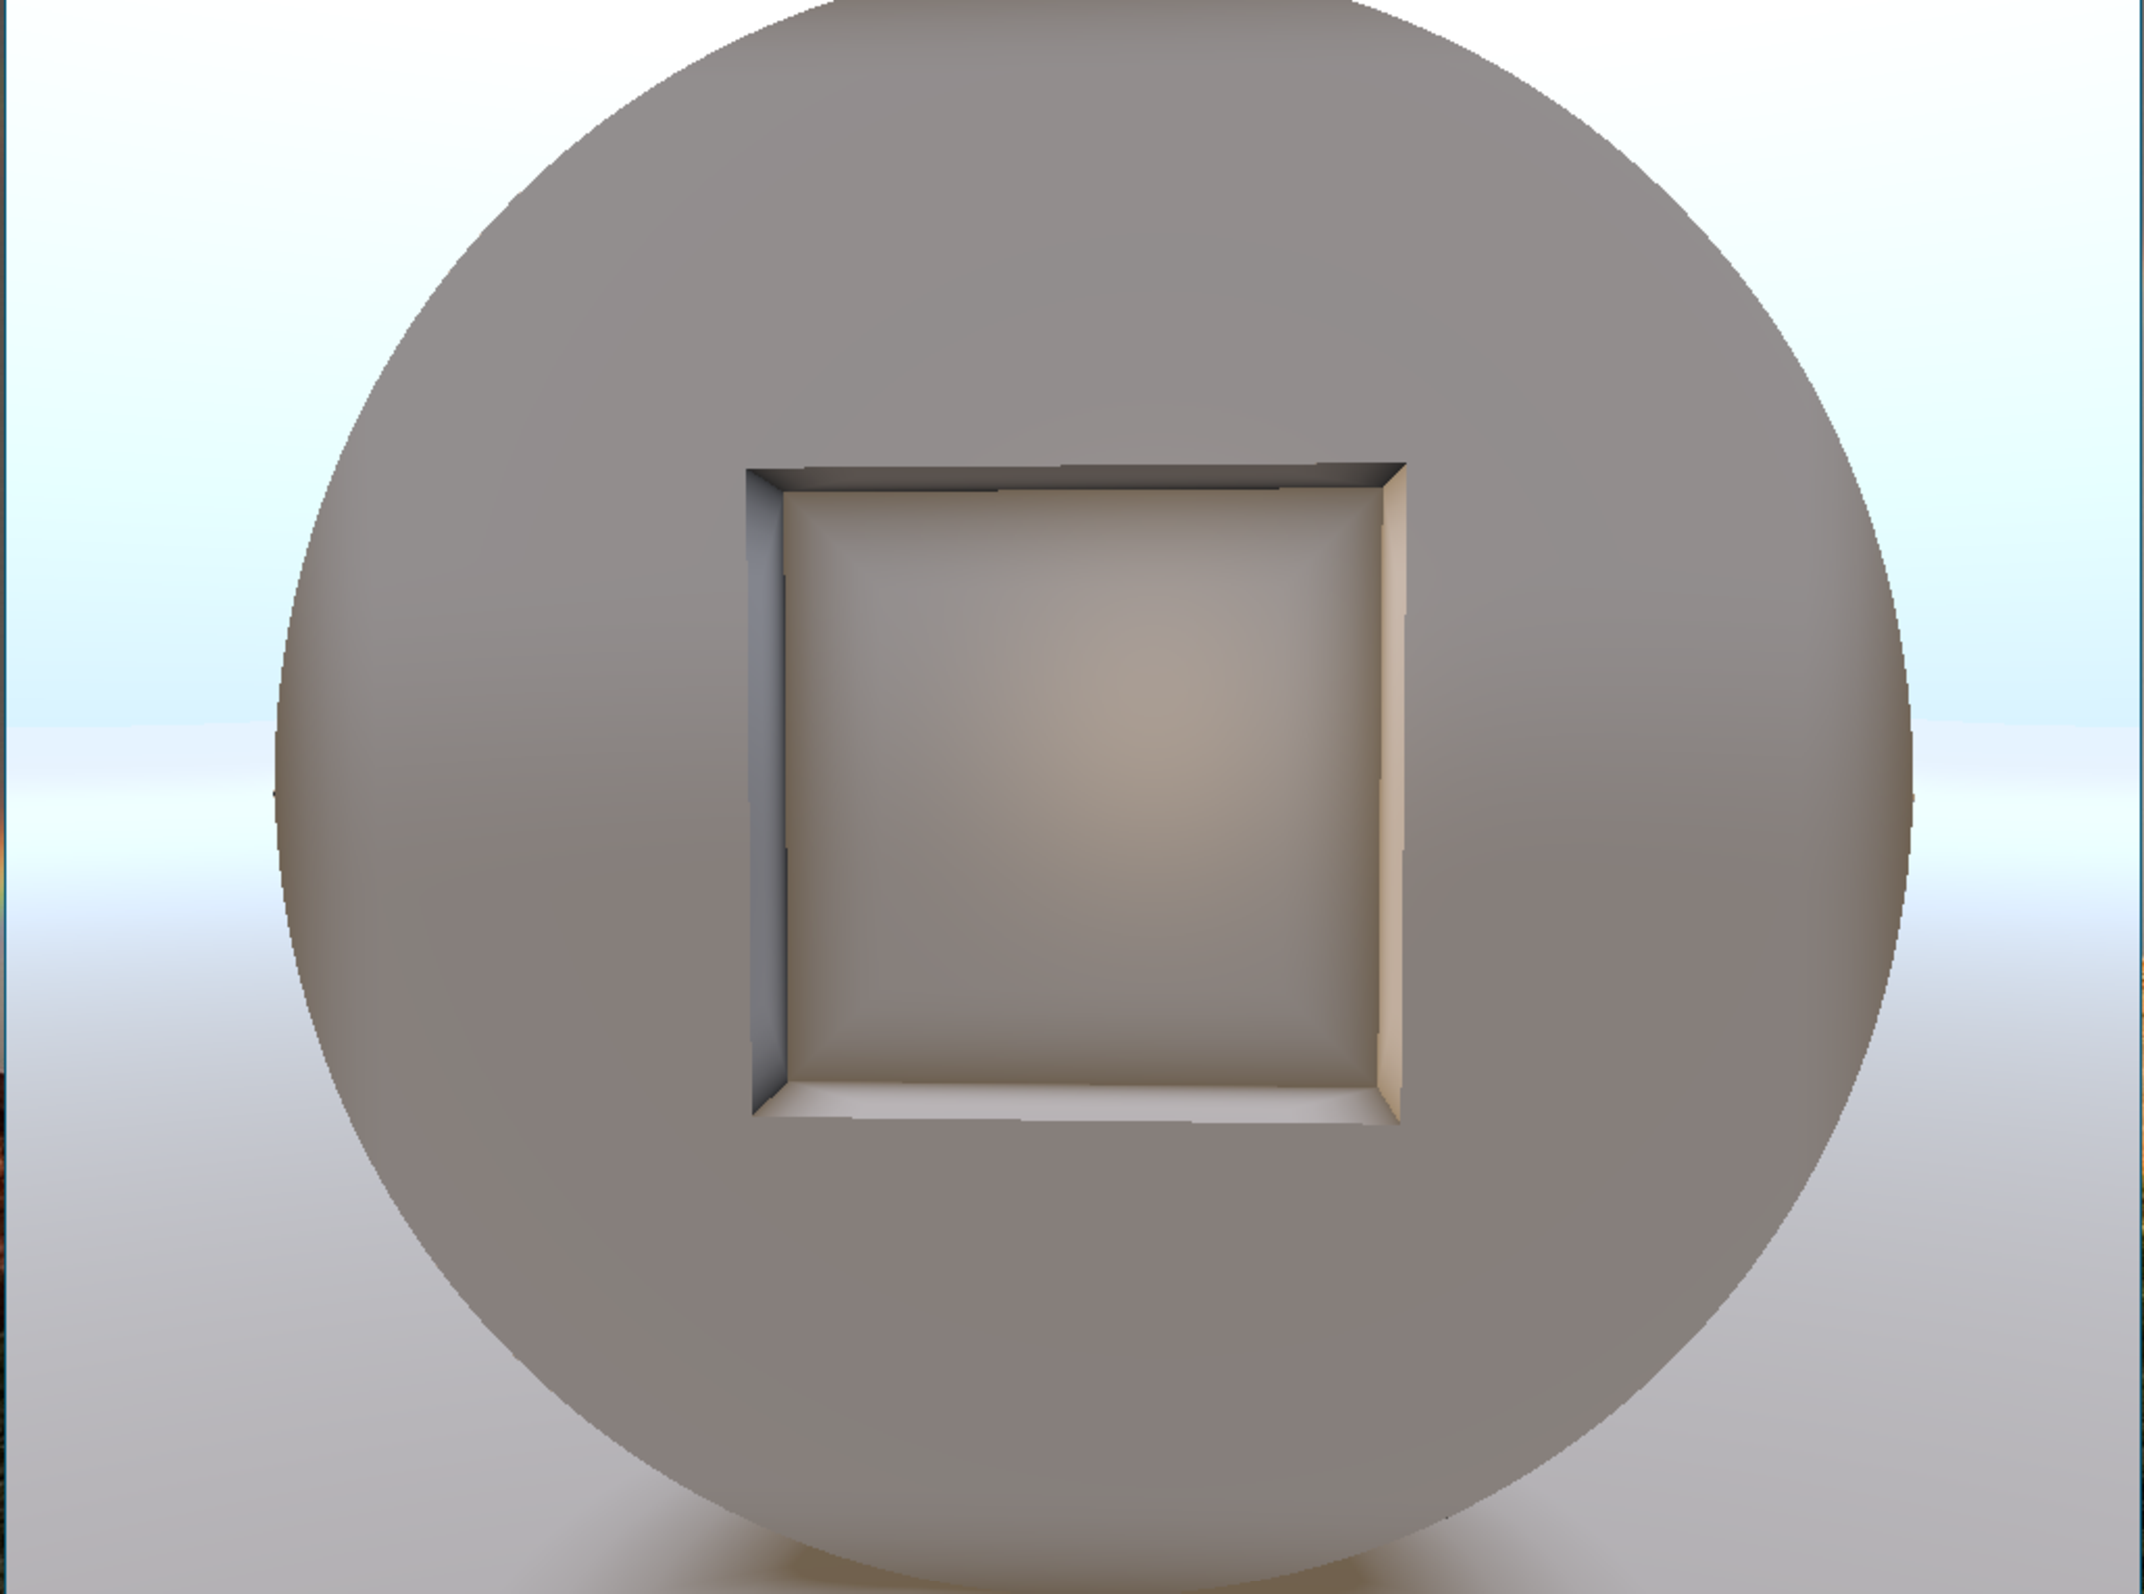
\includegraphics[width=0.5\textwidth]{img/sphere_tracing_subtraction.pdf}
    \caption{Mehrfache Subtraktion: In einem ersten Schritt wird in der
        Hälfte der Kugel ein Würfel von der Kugel subtrahiert. Der Würfel
        hat dieselbe Höhe wie die Kugel. In einem zweiten Schritt wird ein
        wesentlich kleinerer Würfel von der Halbkugel
        subtrahiert.\protect\footnotemark}\label{
        fig:implicit_surfaces_ops_subtraction}
\end{figure}
\footnotetext{Eigene Darstellung}

\subsubsection{Intersektion}
\label{ssubsec:implicit_surfaces_ops_intersection}

Die Intersektion zweier impliziter Oberflächen $A$ und $B$ wird
von~\cite{hart_sphere_1994} als minimale Distanz der jeweiligen
vorzeichenabhängigen  Distanzfunktion $f_{A}$ respektive $f_{B}$
definiert~\parencite[S. 532]{hart_sphere_1994}:

\begin{gather}
    d(\bm{x}, A \cap B) \geq \max(f_{A}(\bm{x}), f_{B}(\bm{x}))
\end{gather}

Dabei stellt $\bm{x}$ den abzutastenden Punkt im Raum dar.
